\documentclass{standalone}
\usepackage{standalone}

\begin{document}

\subsection{Edge Analysis}
Before detectining edges we first applied a threshold value to the estimated license plates (Figure \ref{fig:ThresholdCanny}).
\begin{figure}
\begin{subfigure}{.5\textwidth}
  \centering
  
\includegraphics[width=.8\linewidth]{./img/sample/stage7-1.jpg}
\end{subfigure}
\begin{subfigure}{.5\textwidth}
  \centering
  
\includegraphics[width=.8\linewidth]{./img/sample/stage7-2.jpg}
\end{subfigure}
\begin{subfigure}{.5\textwidth}
  \centering
  
\includegraphics[width=.8\linewidth]{./img/sample/stage7-3.jpg}
\end{subfigure}
\begin{subfigure}{.5\textwidth}
  \centering
  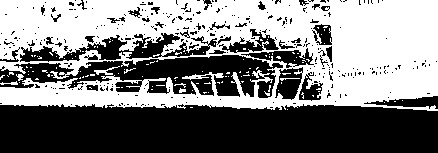
\includegraphics[width=.8\linewidth]{./img/sample/stage7-4.jpg}
\end{subfigure}
\caption{Applying threshold before Canny edge detection.}
\label{fig:ThresholdCanny}
\end{figure}

Canny Edge Detection is a popular edge detection algorithm. OpenCV has a direct function to it. We used the default function OpenCV provides to detect all edges of the localized estimated license plate image (Figure \ref{fig:CannyEdges}). 
\begin{lstlisting}[language=Python]
canny = cv2.Canny(img, 100, 200, L2gradient=True)
\end{lstlisting}

\begin{figure}
\begin{subfigure}{.5\textwidth}
  \centering
  
\includegraphics[width=.8\linewidth]{./img/sample/stage8-1.jpg}
  \caption{Edges of \ref{fig:FirstExtracted}}
\end{subfigure}
\begin{subfigure}{.5\textwidth}
  \centering
  
\includegraphics[width=.8\linewidth]{./img/sample/stage8-2.jpg}
  \caption{Edges of \ref{fig:FirstExtracted}}
\end{subfigure}
\begin{subfigure}{.5\textwidth}
  \centering
  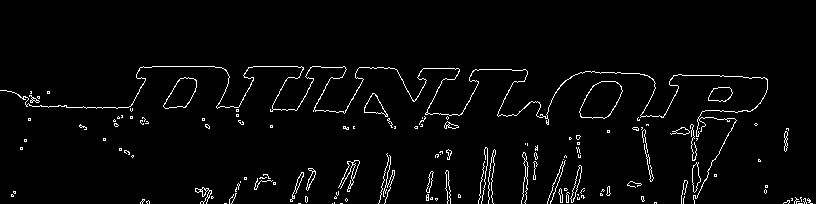
\includegraphics[width=.8\linewidth]{./img/sample/stage8-3.jpg}
  \caption{Edges of \ref{fig:FirstExtracted}}
\end{subfigure}
\begin{subfigure}{.5\textwidth}
  \centering
  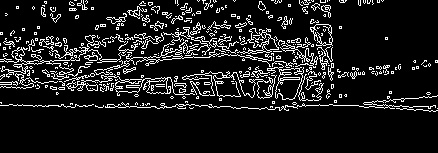
\includegraphics[width=.8\linewidth]{./img/sample/stage8-4.jpg}
  \caption{Edges of \ref{fig:FirstExtracted}}
\end{subfigure}
\caption{Result of Canny edge detecton algorithm.}
\label{fig:CannyEdges}
\end{figure}



\end{document}